

\begin{center}
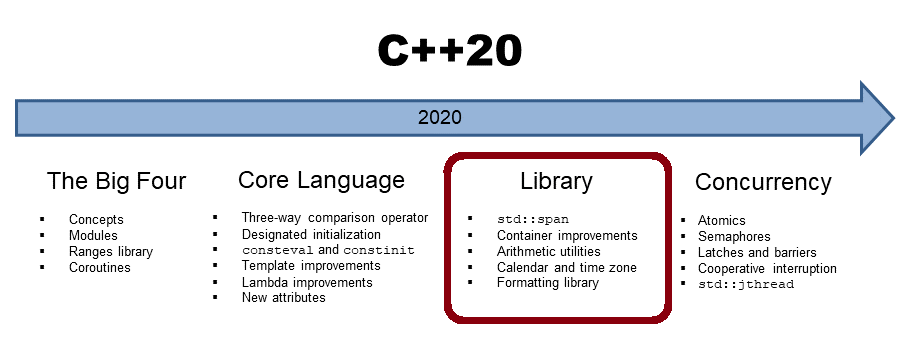
\includegraphics[width=1.0\textwidth]{content/2/chapter3/images/6.png}\\
\end{center}

\subsubsubsection{3.3.1\hspace{0.2cm} std::span}

A std::span represents an object that can refer to a contiguous sequence of objects. A std::span, sometimes also called a view, is never an owner. This view can be a C-array, a std::array, a pointer with a size, or a std::vector. A typical implementation of a std::span needs a pointer to its first element and a size. The main reason for having a std::span is that a plain array will decay to a pointer if passed to a function; therefore, its size is lost. std::span automatically deduces the size of an array, a std::array, or a std::vector. If you use a pointer to initialize a std::span, you have to provide the size in the constructor.

\noindent
std::span as function argument
\begin{lstlisting}[style=styleCXX]
void copy_n(const int* src, int* des, int n){}

void copy(std::span<const int> src, std::span<int> des){}

int main(){
	
	int arr1[] = {1, 2, 3};
	int arr2[] = {3, 4, 5};
	
	copy_n(arr1, arr2, 3);
	copy(arr1, arr2);
	
}
\end{lstlisting}

Compared to the function copy\_n, copy doesn’t need the number of elements. Hence, a common cause of errors is gone with std::span<T>.

\subsubsubsection{3.3.2\hspace{0.2cm} Container Improvements}

C++20 has many improvements regarding containers of the Standard Template Library. First of all, std::vector and std::string have constexpr constructors and can, therefore, be used at compile time. All standard library containers support consistent container erasure and the associative containers support a contains member function. Additionally, std::string allows checking for a prefix or suffix.

\subsubsubsection{3.3.3\hspace{0.2cm} Arithmetic Utilities}

The comparison of signed and unsigned integers is a subtle cause of unexpected behavior and, therefore, of bugs. Thanks to the new safe comparison functions for integers, std::cmp\_*, a subtle source of bugs is gone.

\noindent
Safe comparison of integers
\begin{lstlisting}[style=styleCXX]
int x = -3;
unsigned int y = 7;

if (x < y) std::cout << "expected";
else std::cout << "not expected"; // not expected

if (std::cmp_less(x, y)) std::cout << "expected"; // expected
else std::cout << "not expected";
\end{lstlisting}

Additionally, C++20 includes mathematical constants, including e, π, or ϕ in the namespace std::numbers.

The new bit manipulation enables accessing individual bits and bit sequences, and reinterpreting them.

\noindent
Accessing individual bits and bit sequences
\begin{lstlisting}[style=styleCXX]
std::uint8_t num= 0b10110010;

std::cout << std::has_single_bit(num) << '\n'; // false
std::cout << std::bit_width(unsigned(5)) << '\n'; // 3
std::cout << std::bitset<8>(std::rotl(num, 2)) << '\n'; // 11001010
std::cout << std::bitset<8>(std::rotr(num, 2)) << '\n'; // 10101100
\end{lstlisting}

\subsubsubsection{3.3.4\hspace{0.2cm} Calendar and Time Zones}

The \href{https://en.cppreference.com/w/cpp/chrono}{chrono library} from C++11 is extended with calendar and time-zone functionality. The calendar consists of types which represent a year, a month, a day of the week, and an n-th weekday of a month. These elementary types can be combined, forming complex types such as for example yea\_month, year\_month\_day, year\_month\_day\_last, year\_month\_weekday, and year\_month\_weekday\_last. The operator “/” is overloaded for the convenient specification of time points. Additionally, we get new literals: d for a day and y for a year.

Time points can be displayed in various time zones. Due to the extended chrono library, the following use cases are now trivial to implement:

\begin{itemize}
\item 
representing dates in specific formats

\item 
get the last day of a month

\item 
get the number of days between two dates

\item 
printing the current time in various time zones
\end{itemize}

The following program presents the local time in different time zones.

\noindent
The local time in various time zones
\begin{lstlisting}[style=styleCXX]
using namespace std::chrono;

auto time = floor<milliseconds>(system_clock::now());
auto localTime = zoned_time<milliseconds>(current_zone(), time);
auto berlinTime = zoned_time<milliseconds>("Europe/Berlin", time);
auto newYorkTime = zoned_time<milliseconds>("America/New_York", time);
auto tokyoTime = zoned_time<milliseconds>("Asia/Tokyo", time);

std::cout << time << '\n'; // 2020-05-23 19:07:20.290
std::cout << localTime << '\n'; // 2020-05-23 21:07:20.290 CEST
std::cout << berlinTime << '\n'; // 2020-05-23 21:07:20.290 CEST
std::cout << newYorkTime << '\n'; // 2020-05-23 15:07:20.290 EDT
std::cout << tokyoTime << '\n'; // 2020-05-24 04:07:20.290 JST
\end{lstlisting}

\subsubsubsection{3.3.5\hspace{0.2cm} Formatting Library}

The new formatting library provides a safe and extensible alternative to the printf functions. It’s intended to complement the existing I/O streams and reuse some of its infrastructure, such as overloaded insertion operators for user-defined types.

\begin{lstlisting}[style=styleCXX]
std::string message = std::format("The answer is {}.", 42);
\end{lstlisting}

std::format uses Python’s syntax for formatting. The following examples show a few typical use cases:

\begin{itemize}
\item 
Format and use positional arguments

\begin{lstlisting}[style=styleCXX]
std::string s = std::format("I'd rather be {1} than {0}.", "right", "happy");
// s == "I'd rather be happy than right."
\end{lstlisting}

\item 
Convert an integer to a string in a safe way

\begin{lstlisting}[style=styleCXX]
memory_buffer buf;
std::format_to(buf, "{}", 42); // replaces itoa(42, buffer, 10)
std::format_to(buf, "{:x}", 42); // replaces itoa(42, buffer, 16)
\end{lstlisting}

\item 
Format user-defined types

\end{itemize}

